\chapter{User adaptation and Transfer Learning}
\label{chapter:dm-tl}

In the previous chapter, we introduced \acrfull{RL} solutions for the \acrfull{DM}. For that, we cast the problem as an \idx{agent}, the \gls{DM}, interacting with an \idx{environment}: the \idx{user}.
In classic approaches, we actually consider the \idx{environment} as any potential \idx{user}, and then learn a policy able to converse with this \textit{generic} \idx{user}. This approach assumes all \idx{user}s to adopt the same dialoguing behaviour, although this not necessarily the case.
%!TU: question (vache) pour la soutenance: mais ne serait-il pas plus simple de coder le profil de l'utilisateur dans l'etat du dialogue ?
%NC: ça existe. Mon avis est qu'il faut savoir à l'avance les paramètres à utiliser pour disciminer les users. Et puis determiner ces paramètres en live c'est peut etre moins simple. On peut faire le rapprochement avec model based et model free rl. Si le model est facile, il faut faire du model base, si la Q function est facile, il faut faire du model free. Pour l'user adapt, comme l'humain n'est pas facile, on prefererait optimiser la Q function directement, au lieu de chercher le model de l'humain.
%
%So there are two explanations to such restricting \idx{model}s. In one hand, the designer may consider the \idx{dialogue} task so simple such that all \idx{user}s will react in the exact same way when dialoguing with a machine. For example, communicating a social security number to a vocal server. In the end, this statement may be true for proof of concepts and easy tasks but in the general case, it is biased. On the other hand,
The designer may choose to represent all \idx{user}s as the same unique entity to accelerate the learning of the \gls{DM}. It is a fair argument indeed, but it may impact negatively the overall quality of the \idx{dialogue}. In consequence, in the following, we present solutions to overcome this limitation. We adopt the \acrfull{TL} framework~\parencite{LazaricSurvey,taylor2009transfer} where the objective consists in improving the learning of a target task, thanks to the knowledge obtained from a set of similar source tasks. In \idx{dialogue}, we usually associate a task with a unique \idx{user} or a domain. Then, the \gls{DM} communicates with an unknown \idx{user}/domain based on its past experience with other \idx{user}s/domains. One could also consider a setup where there is a single \idx{user} with several communication channels making different tasks. For example, talking through the phone, VoIP, or face to face. That being said, in this manuscript, we consider one \idx{user} by task.

\section{The problem of Transfer Learning}

As stated in \textcite{LazaricSurvey}, \gls{TL} leverages the knowledge collected from a number of different tasks to improve the learning performance in new tasks. In our case, a \textit{task} is defined as "dialoguing with a \idx{user} $u$" and as we saw in previous chapter, modelled as an \gls{MDP}. We denote this \gls{MDP} as $u =\left\langle \cS_{u}, \cA_{u}, \transition_{u}, \reward_{u}\right\rangle$\footnote{By abusing the notations, the \idx{user} $u$, its \gls{MDP} and the task describe the same concept.}. The \gls{TL} vocabulary is the following\footnote{The notation and the description of \gls{TL} are largely inspired from the survey \textcite{LazaricSurvey}}: the \textit{domain} of the task $u$ is the state-action space $\cS_{u} \times \cA_{u}$; The \textit{space of tasks} is the set of potential \idx{user}s $\users = \{u_j\}_{j\in[0,M]}$; The \textit{\idx{environment}} $\rE=\langle\users, \Omega\rangle$, is denoted as the the probability distribution $\Omega$ over the space of tasks. The \idx{environment} $\rE$ fully describes the problem: the \gls{DM} must find the best strategy to adopt with a target \idx{user} $u_t$ drawn from the distribution $\Omega$. In order to operate this learning quickly, the \gls{DM} has access to the knowledge gathered previously with source \idx{user}s $\users_{\!s} =\{u_s\}_{s\in[0,M_s]}  \sim \rE$ drawn from the environment. In a sense, we can see the \gls{TL} problem as a \gls{SL} problem where already encountered \idx{user}s stand for the learning base and the new \idx{user} is part of the test base. The idea is then to construct a general \idx{model}, that returns a \gls{DP} given a \idx{user}, which is able to generalise across unseen \idx{user}s. In what follows, the adjectives source/target may be combined to other notions. For example, a source policy $\policy_s$ denotes a policy learnt with a source \idx{user} $u_s$, the target \idx{transition}s $\{(s_{\indextransition},a_{\indextransition},r_{\indextransition}',s_{\indextransition}')\}_{{\indextransition}\in \T_t}$ denote the \idx{transition}s gathered with the target \idx{user} $u_t$.

Let $\cK$ be the space of the knowledge spawned by all \idx{user}s. As we do not access to the whole space, the target user knowledge may be a part of it and this is where \gls{TL} comes in. Two distinct phases constitute a \gls{TL} algorithm: the \textit{knowledge-\idx{transfer}} phase that extracts from $\cK$ the relevant subset of knowledge for the target task and the \textit{learning} phase that constructs a policy accordingly. The process may be strictly sequential or cyclic. In the literature, \gls{TL} approaches differ following three criterions: the type of knowledge \idx{transfer}red, the objectives, and the setting.

\paragraph{The type of the knowledge} Three types of \idx{transfer} are reported in the general \gls{TL} literature: the \idx{transfer} of \idx{transition}s where the interactions with previous tasks are used to learn the policy for a target task~\parencite{sunmola2006model,lazaric2008,taylor2008transferring}; the \idx{transfer} of representations, for example state features\index{feature}~\parencite{ferguson2006proto,mahadevan2007proto,ferrante2008transfer}, action space~\parencite{sherstov2005improving}, some layers of a \gls{NN} or temporal abstractions for policies~\parencite{sutton1999options}; the \idx{transfer} of parameters, including meta parameters (learning rate, discount factor etc), $\Q$-function initialisation~\parencite{torrey2005using} or even source policy \idx{transfer} ~\parencite{taylor2007transfer}.

\paragraph{The objectives}

In \gls{RL}, we can distinguish three objectives that represent the performances of an \idx{agent}: the \idx{jumpstart} performance\footnote{Also know as bootstrap or coldstart performance.}, where we measure how well an \idx{agent} performs in the very first interactions with the \idx{environment} (the \idx{user});
the learning performance, where we measure how well the \idx{agent} performs when improving its current policy; finally, the \gls{TL} \idx{agent} monitors an additional objective called asympotic performance, which measure the performances when the target dataset contains all the knowledge needed to compute the optimal policy.

The three objectives are displayed in the green circles of \Cref{fig:objectives}. \gls{TL} \idx{agent} may optimise one, two or three of those objectives. A phenomenon we want to avoid, called negative \idx{transfer}, is when the performances of an agent are better without transfer. A typical instance of this phenomena may occur when \idx{transfer}ring \idx{transition}s. Importing the source \idx{transition}s may help to learn an initial generic policy improving jumpstart and learning performances, but if the \idx{transition}s are too far from the target \idx{environment}, and the learning algorithm has no mechanism to forget this knowledge, the target \idx{model} will be biased and the asymptotic performance will be affected.

\begin{figure}
    \begin{center}
        \subfloat[jumpstart performance]{
        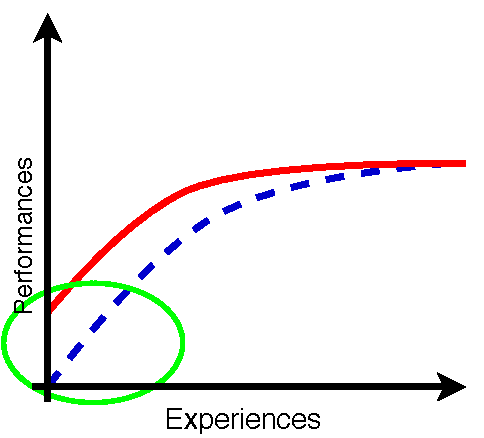
\includegraphics[width=0.33\textwidth]{sources/dm-tl/objectives-jumpstart}
        \label{fig:objectives-jumpstart}
        }
        \subfloat[Learning performance]{
        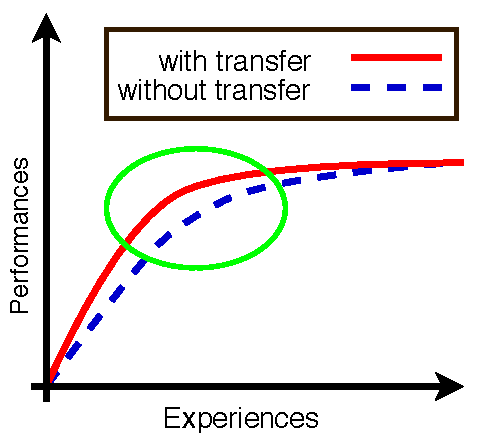
\includegraphics[width=0.33\textwidth]{sources/dm-tl/objectives-learn}
        \label{fig:objectives-learn}
        }
        \subfloat[Asymptotic performance]{
        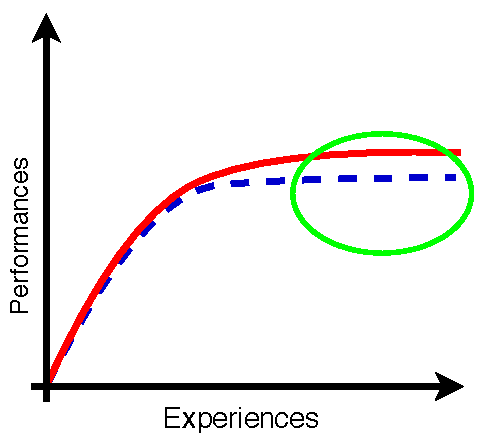
\includegraphics[width=0.33\textwidth]{sources/dm-tl/objectives-asymptote}
        \label{fig:objectives-asymptote}
        }
        \caption{Objectives of Transfert Learning~\parencite{langley2006,LazaricSurvey}}
        \label{fig:objectives}
    \end{center}
\end{figure}

\paragraph{The setting}

We distinguish \gls{TL} given two setting properties:

\begin{itemize}
    \item whereas the domain $\cS_{u}, \cA_{u}$ is fixed between the tasks. Usually, if the domain is not fixed, \gls{TL} solutions focus on solving a simpler problem where the source task is unique. The difficulty lies in the mapping between those two tasks;
    \item whereas there is only one source task or several. The distinction may be hard to operate as one can consider, for example, a set of different \idx{user}s as a single \textit{average} \idx{user}, hence a single task. So to make things clear, here, we propose three settings:
\begin{itemize}
        \item \textit{mono-task}  where there is only one source task and one target task. The method is a direct mapping between those two tasks;
        \item \textit{generic-task}, where there is only one source task, but that may be several tasks seen as a generic task and there are potentially multiple target tasks;
        \item \textit{multi-task}, where there is several source tasks, and the distinction between tasks is made clear and relevant for the \textit{knowledge-\idx{transfer}} phase. There are potentially multiple target tasks.
\end{itemize}
    Please note that given this description, a method defined for a generic-task setting is not necessarily worse than a method defined for the \textit{multi-task} purpose. On the contrary, methods relying on \textit{mono-task} \idx{transfer} are by definition limited to the tasks.

\end{itemize}

In this thesis, we propose solutions for \idx{user adaptation} \gls{TL} with \textit{fixed domain} and we consider a \textit{generic-task} and a \textit{multi-task} setting.

\section{State-of-the-art of Transfer Learning for Dialogue Systems}

We distinguish two main parts in \gls{TL} for \glspl{DS}. A whole part of the literature tackles the problem of compatibility between different domains. Here the term domain stands for "domain of application" and not the domain $\cS_{u}, \cA_{u}$, even if it is closely related. For example, how to apply a policy learnt for a restaurant reservation application to a hotel reservation application. Please note that in this case, the tasks denote \glspl{MDP} representing different domains and not \idx{user}s (as explained in the previous section). This part will be discussed briefly. The second part of the literature concerns \idx{user adaptation}, which will be further studied in the thesis. Finally, we will discuss a solution for evaluating real-life \idx{dialogue}s with prior knowledge. All methods discussed are listed in \Cref{table:survey}.

\subsection{Cross domain adaptation}

The first application of \gls{TL} to \gls{DM} has been proposed by ~\parencite{Gasic2013} and it was for cross domain \idx{adaptation}.

\paragraph{\cite{Gasic2013}} This approach considers extending a \gls{DP} ability of handling several slots from a basic domain (the source \idx{environment}), including \textit{food-type} slot and the \textit{area} slot for example, to an extended domain (the target \idx{environment}) equipped with an additional unknown slot, the \textit{price-range} slot. \glspl{DM} are \gls{GP} \glspl{DP} ~\parencite{Rasmussen2006-gp-for-machine-learning,Gasic2014-gp-pomdp-dialogue} using a \idx{transition}s dictionary to keep the problem tractable~\parencite{Engel2006-gp-dictonnary}. The \gls{DST} module is implemented using The Bayesian Update of Dialogue State~\parencite{Thomson2009-BUDS-dialogue} for tracking belief states.

First, they propose a novel idea which allows a policy trained in the basic domain to be used in an extended domain: a kernel function that defines the correlation between belief states from different domains. Then, they investigate two solutions in order to quickly adapt to the new domain:

\begin{itemize}
    \item Simply continue the training of the source policy in the extended domain. To that extent, a zero-mean prior is set on the \gls{GP} for the $\Q$-function. The \textit{knowledge-\idx{transfer}} phase consists in including \idx{transition}s from both domains in the dictionary\footnote{It is quite hard to categorise the type of knowledge \idx{transfer}red as \gls{GP} are nonparametric, so the \idx{transition}s represent directly the parameters. But following the author description, it is policy \idx{transfer}.}.
    \item The prior of the mean of the \gls{GP} $\Q$-function in the extended domain is the posterior of the mean from the \gls{GP} $\Q$-function in the basic domain.
\end{itemize}

The authors validate both approaches with human experiments showcasing significant improvements during the \idx{jumpstart} phase.

\paragraph{To go beyond}

Other approaches that go beyond the scope of this thesis have been released in the past few years. In \textcite{Keizer2016-tl-dialogue,Keizer2018-tl-dialogue}, the authors solve the cross-domain problem by casting the \gls{DM} as a multidimensional system. They learn common \idx{transfer}able skills.

A multi-\idx{agent} solution is adopted in \textcite{Chen2018-tl-dialogue}. They learn two types of \idx{agent}, \textit{slot-dependent} and \textit{slot-independent} \idx{agent}s. Rather than \idx{transfer}ing the common knowledge as in \textcite{Keizer2018-tl-dialogue}, they \idx{transfer} \textit{slot-dependent} \idx{agent}s in the target domain.

In \textcite{Ilievski2018-tl-dialogue}, they propose to operate \idx{transfer} using the weights of the \idx{policy}'s \gls{NN} from the source domain to the target domain. But because domains are not the same, they have to extend the \idx{dialogue state} and action spaces of both domains in order to render the \idx{transfer}red knowledge compatible.

\subsection{User adaptation}


%!TU: Remarque
% Ton probleme a une specificite qui n'apparait
% pas dans le TL classique:
% tu transferes d'un ensemble de taches vers une de ces tache
% il y a un cote "local learning" i.e. on apprend un modele multi
% utilisateurs que l'on specialise pour un utilisateur donne.
% Il y certe une perte a cause du biai de transfert, mais il y a un gain
% en terme de variance : la tache source est plus riche en donnees que la
% tache cible.


When the different \idx{user}s denotes the space of tasks, we talk about \idx{user adaptation}. Before listing the state of the art in \idx{user adaptation}, we recall why it is essential.

\paragraph{On the need of \idx{user adaptation}}

\acrfullpl{DM} are usually trained versus \idx{user-model}s~\parencite{eckert1998bigram,first-mdp-sds,levin2000stochastic,these-pietquin,asri2016rnn} , agenda-based \idx{user}-simulator ~\parencite{schatzmann2008statistical, keizer2010parameter} or \idx{dialogue} simulator~\parencite{laroche2017ndg,khouzaimi2017-sim-dialogue}. Initially, \idx{model}s were trained and tested against the same \idx{user-model}.

In \textcite{schatztnann2005-tl-dialogue}, they demonstrated empirically that testing \glspl{DP} trained on poor \idx{user-model} (the bigram model), against more sophisticated \idx{user-model}s (the Levin-model or the Pietquin-model) led to poor performances. Assuming humans are more complex that the finest \idx{user-model}, it is natural to infer that \gls{DM} learnt on \idx{user-model}s may perform poorly in real conditions. Even if the paper focused on the quality of \idx{user-model}s, we see that any \gls{DM} cannot be used for any target \idx{user-model} (or human), thus a \textit{knowledge-\idx{transfer}} phase is essential. The same idea applies if the target \idx{environment} is a parametric \idx{user-model} simulating different kind of \idx{user}s. In \textcite{lemon2007-tl-dialogue}, they learnt different policies against \idx{user-model}s with 2 types of variations: \idx{user} type (Cooperative/Uncooperative), and noise conditions (High/Low). Even if the policies trained in high-noise conditions  generally perform better than those trained for low-noise conditions, no policies is the best fit for all \idx{user-model}s, thus a \textit{knowledge-\idx{transfer}} phase is also needed. While those two examples are not \gls{TL} strictly speaking, they clearly show that \idx{user} \idx{adaptation} is essential. There are indeed a handful of published works in this domain that we survey in the following paragraphs.

\paragraph{\cite{casanueva2015-tl-dialogue}} In this paper, they propose to personalise \glspl{DS} to different speakers suffering from dysarthria. Users are simulated\index{user-model} and their respective dysarthia seriousness is adjusted using the \gls{ASR} module. As in \textcite{Gasic2013}, \glspl{GP} are \gls{GP} policies; they are learnt with Deterministic Training Conditional. In order to adapt the target policy to new \idx{user}s, they introduce two \textit{knowledge-\idx{transfer}} solutions which adress respectively two issues: which source to \idx{transfer} from and how to weight the \idx{transition}s \idx{transfer}red from multiple sources.

To select the source to \idx{transfer}, they introduce a similarity function between speakers (along with 3 different speaker features\index{feature}) which is a Radial Basis Function kernel. They also pick the most similar \idx{transition}s to the target speaker to reduce the amount of \idx{transfer}red data.

In order to weight the \idx{transition}s \idx{transfer}red, they reduce the covariance of two \idx{transition}s where the source and target speakers are similar. They make it possible by extending the \idx{transition}s with the speaker features\index{features}. Then, they extend the \gls{GP} kernel defined in the state-action space with the Radial Basis Function kernel in the speaker space previously mentioned. The authors show that this method outperforms the source selection.

To design the target policy\footnote{Please note that there is no \textit{learning} phase strictly speaking since \gls{GP} \gls{ML} algorithms use lazy learning (instead of learning a model with the data, then doing inferences with the model, the data is directly used during the inferences).}, they propose to divide the \idx{transfer}red \idx{transition}s in two sets. The first set allows one to learn the posterior of the mean of the source \gls{GP} $\Q$-function used as the prior in the target context, which is one of the solutions proposed in \textcite{Gasic2013}. The second set is used to initialise the set of points needed to compute the parameters of the target \gls{GP} $\Q$-function.

\paragraph{\cite{Genevay2016}} The method proposed in this paper embraces the problem of \idx{user} \idx{adaptation} by \idx{transfer}ring the \idx{transition}s of previous encountered \idx{user}s to learn the target policy with \gls{FTQ}. An algorithm is also proposed to pick the source set of \idx{transition}s using \gls{UCB}. Finally, Density-Based, a way of picking the relevant \idx{transition}s in the source set for the target task, is also introduced. The overall framework is tested on the \acrfull{NDG}. The main limitation is the following: as the number of source user grows, the number of arms for the UCB algorithm grows too. It becomes impracticable to test at least once each arm with the target user. One of the contributions we propose in this thesis fixes this problem, hence for more details, please refer to \Cref{chapter:sigdial}.

\paragraph{\cite{carrara2017online}} In this work, detailed \Cref{chapter:sigdial}, we extend \textcite{Genevay2016} in order to handle a larger pool of source policies. We propose a \idx{clustering} approach and test it on \idx{handcrafted user}s as well as \idx{human-model user}s.


\paragraph{\cite{Mo2018-tl-dialogue-PETAL}} The approach introduced in this work, called PETAL, \idx{transfer}s parameters to process \idx{user} \idx{adaptation} with a real-world coffee ordering dataset. To that extent, they model the $\Q$-function of the target policy as the sum of a common $\Q$-function learnt using data gathered on several source \idx{user}s and a personalised $\Q$-function learnt on the target \idx{transition}s. A weight vector $w$ representing the influence of the common $\Q$-function over the personalised $\Q$-function is extracted from the same data. Finally, they construct a \gls{DST} module that is a function mapping dialogue history to belief state using a state-projection matrix denoted $M$. This matrix is also learnt with the source \idx{transition}s. In the end, they \idx{transfer} three parameters set to learn the target policy: the parameters of the common $\Q$-function, the matrix $M$ and the vector $w$. The authors use a \gls{SARSA}~\parencite{rummery1994line} algorithm to regress the target $\Q$-function. They validate the approach on both simulated and real work data comparing several baselines (including~\textcite{casanueva2015-tl-dialogue}, \textcite{Genevay2016} and \textcite{Gasic2013} modified for \idx{user} \idx{adaptation}).

\paragraph{\cite{carrara2018safe}} We introduce an approach based on the \idx{transfer} of a \idx{safe policy} learnt on the complete pool of source \idx{user}s. This solution is discussed in \Cref{chapter:slsp}.

\subsection{An aside on dialogue evaluation}

On real \gls{SDS} problems, it is usually hard to infer on-the-fly if the \idx{dialogue} ended well. For example, in a task-completion problem, during the \idx{dialogue}, the system cannot know if a slot has been understood thus it is impossible to infer if the task is a success or not. If the recognition score is high, there is more chance that the system understood correctly, but still, it is not a perfect measure. To that extent, \textcite{elasri2014-tl-dialogue} proposes to \idx{transfer} a reward function inferred from a set of evaluated \idx{dialogue}s (by experts or other evaluation techniques). The authors learn this function using Inverse Reinforcement Learning with the reward shaping algorithm proposed in \textcite{ElAsri2012-reward-shapping-dl}. They learn the target policy using \gls{LSPI} on a target \idx{environment} equipped with the learnt reward function.

\begin{table*}
    \centering
    \resizebox{\textwidth}{!}{
    \begin{tabular}{llll}
        \hline
        & Knowledge & Setting & Metric \\ \hline

        \hline
        \textbf{cross domain} &&&\\
        \hline
        \cite{Gasic2013}& parameter (\idx{transition}s/policy)  & \makecell[l]{mono-task\\ cross-domain} & all         \\
        \cite{Keizer2018-tl-dialogue}& parameter (policy)& \makecell[l]{generic-task\\ cross-domain} & all      \\
        \cite{Chen2018-tl-dialogue}& parameter (policy) & \makecell[l]{generic-task\\ cross domain} & all       \\
        \cite{Ilievski2018-tl-dialogue}& parameter (policy) & \makecell[l]{mono-task\\ cross-domains }& all      \\
        \hline
        \textbf{\idx{user} \idx{adaptation}} &&&\\
        \hline
        \cite{casanueva2015-tl-dialogue}& parameter (\idx{transition}s/policy) & \makecell[l]{multi-task\\ fixed domain} & all         \\
        \cite{Genevay2016}& \makecell[l]{\idx{transition}s \\ parameter (policy)} & \makecell[l]{multi-task\\ fixed domain }& all   \\
        \cite{carrara2017online}& \makecell[l]{\idx{transition}s \\ parameter (policy)} & \makecell[l]{multi-task\\ fixed domain} & all   \\
        \cite{Mo2018-tl-dialogue-PETAL}& parameter ($\Q$-function, \gls{DST}) & \makecell[l]{generic-task\\ fixed domain }& all        \\
        \cite{carrara2018safe}& parameter (policy) & \makecell[l]{generic-task\\ fixed domain} & all   \\
        \hline
        \textbf{dialogue evaluation} &&&\\
        \hline
        \cite{elasri2014-tl-dialogue}& representation (reward function) & \makecell[l]{generic-task\\ fixed domain} & all        \\
        \hline

    \end{tabular}
    }
    \caption{Transfer Learning for Dialogue Systems}
    \label{table:survey}
\end{table*}
